%%%
\chapter{Figures and Tables}

\section{Figures}
You can import external graphics\index{graphics} using package graphicx. The most important command is `includegraphics'. LaTeX itself treats the image like normal text, i.e. as a box of certain height and width. The `graphicx' package documentation list the options width and height, as well as others (Figure~\ref{fig:Nature-1}). Using pdflatex several graphics formats are supported: pdf, png and jpg. Modern installations of LaTeX\index{Latex} can use eps files as well, but indirectly.

You can convert EPS to PDF with the epstopdf utility, included in package of the same name. This tool is actually called by pdflatex to convert EPS files to PDF in the background when the graphicx package is loaded. This process is completely invisible to the user. LaTeX in dvi-mode supports only eps-files. 

See Figure~\ref{fig:Nature-2}. 

\begin{figure}[b]
	\centering
	\includegraphics[width=0.45\linewidth]{Nature-1}
	\caption{Nature-1.}
	\label{fig:Nature-1}
\end{figure}

\begin{figure}
	\centering
	\includegraphics[width=0.4\linewidth]{Nature-2}
	\caption{Nature-2.}
	\label{fig:Nature-2}
\end{figure}

\begin{figure}[tbp]
	\centering
	\begin{subfigure}[b]{0.45\textwidth}
		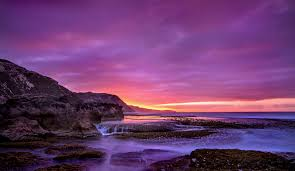
\includegraphics[width=\textwidth]{nature-1}
		\caption{}
		\label{fig:n1}
	\end{subfigure}
	\qquad
	\begin{subfigure}[b]{0.45\textwidth}
		
\includegraphics[width=0.9\textwidth]{nature-2}
		\caption{}
		\label{fig:n2}
	\end{subfigure}
	\caption{Two figures: Nature-1 and nature-2.}\label{fig:figs}
\end{figure}

\section{Tables}
Tables are a common feature in academic writing, often used to summarize research results. Mastering the art of table construction in LaTeX is therefore necessary to produce quality papers\index{papers} and with sufficient practice one can print beautiful tables of any kind.

Keeping in mind that LaTeX is not a spreadsheet, it makes sense to use a dedicated tool to build tables and then to export these tables into the document. Basic tables are not too taxing, but anything more advanced can take a fair bit of construction; in these cases, more advanced packages can be very useful. However, first it is important to know the basics. See sample table~\ref{tab:This table shows some data}.

\begin{table}
	\centering
	\caption{This table shows some data.}
	\label{tab:This table shows some data}
	\begin{tabular}{llr}
		\hline
		\multicolumn{2}{c}{Item} \\
		\cline{1-2}
		Animal    & Description & Price (\$) \\
		\hline
		Gnat      & per gram    & 13.65      \\
		& each        & 0.01       \\
		Gnu       & stuffed     & 92.50      \\
		Emu       & stuffed     & 33.33      \\
		Armadillo & frozen      & 8.99       \\
		\hline
	\end{tabular}
\end{table}
















